% Options for packages loaded elsewhere
\PassOptionsToPackage{unicode}{hyperref}
\PassOptionsToPackage{hyphens}{url}
%
\documentclass[
]{book}
\usepackage{amsmath,amssymb}
\usepackage{lmodern}
\usepackage{ifxetex,ifluatex}
\ifnum 0\ifxetex 1\fi\ifluatex 1\fi=0 % if pdftex
  \usepackage[T1]{fontenc}
  \usepackage[utf8]{inputenc}
  \usepackage{textcomp} % provide euro and other symbols
\else % if luatex or xetex
  \usepackage{unicode-math}
  \defaultfontfeatures{Scale=MatchLowercase}
  \defaultfontfeatures[\rmfamily]{Ligatures=TeX,Scale=1}
\fi
% Use upquote if available, for straight quotes in verbatim environments
\IfFileExists{upquote.sty}{\usepackage{upquote}}{}
\IfFileExists{microtype.sty}{% use microtype if available
  \usepackage[]{microtype}
  \UseMicrotypeSet[protrusion]{basicmath} % disable protrusion for tt fonts
}{}
\makeatletter
\@ifundefined{KOMAClassName}{% if non-KOMA class
  \IfFileExists{parskip.sty}{%
    \usepackage{parskip}
  }{% else
    \setlength{\parindent}{0pt}
    \setlength{\parskip}{6pt plus 2pt minus 1pt}}
}{% if KOMA class
  \KOMAoptions{parskip=half}}
\makeatother
\usepackage{xcolor}
\IfFileExists{xurl.sty}{\usepackage{xurl}}{} % add URL line breaks if available
\IfFileExists{bookmark.sty}{\usepackage{bookmark}}{\usepackage{hyperref}}
\hypersetup{
  pdftitle={Exploring Ecological Data},
  pdfauthor={Dr Ellen Bell},
  hidelinks,
  pdfcreator={LaTeX via pandoc}}
\urlstyle{same} % disable monospaced font for URLs
\usepackage{color}
\usepackage{fancyvrb}
\newcommand{\VerbBar}{|}
\newcommand{\VERB}{\Verb[commandchars=\\\{\}]}
\DefineVerbatimEnvironment{Highlighting}{Verbatim}{commandchars=\\\{\}}
% Add ',fontsize=\small' for more characters per line
\usepackage{framed}
\definecolor{shadecolor}{RGB}{248,248,248}
\newenvironment{Shaded}{\begin{snugshade}}{\end{snugshade}}
\newcommand{\AlertTok}[1]{\textcolor[rgb]{0.94,0.16,0.16}{#1}}
\newcommand{\AnnotationTok}[1]{\textcolor[rgb]{0.56,0.35,0.01}{\textbf{\textit{#1}}}}
\newcommand{\AttributeTok}[1]{\textcolor[rgb]{0.77,0.63,0.00}{#1}}
\newcommand{\BaseNTok}[1]{\textcolor[rgb]{0.00,0.00,0.81}{#1}}
\newcommand{\BuiltInTok}[1]{#1}
\newcommand{\CharTok}[1]{\textcolor[rgb]{0.31,0.60,0.02}{#1}}
\newcommand{\CommentTok}[1]{\textcolor[rgb]{0.56,0.35,0.01}{\textit{#1}}}
\newcommand{\CommentVarTok}[1]{\textcolor[rgb]{0.56,0.35,0.01}{\textbf{\textit{#1}}}}
\newcommand{\ConstantTok}[1]{\textcolor[rgb]{0.00,0.00,0.00}{#1}}
\newcommand{\ControlFlowTok}[1]{\textcolor[rgb]{0.13,0.29,0.53}{\textbf{#1}}}
\newcommand{\DataTypeTok}[1]{\textcolor[rgb]{0.13,0.29,0.53}{#1}}
\newcommand{\DecValTok}[1]{\textcolor[rgb]{0.00,0.00,0.81}{#1}}
\newcommand{\DocumentationTok}[1]{\textcolor[rgb]{0.56,0.35,0.01}{\textbf{\textit{#1}}}}
\newcommand{\ErrorTok}[1]{\textcolor[rgb]{0.64,0.00,0.00}{\textbf{#1}}}
\newcommand{\ExtensionTok}[1]{#1}
\newcommand{\FloatTok}[1]{\textcolor[rgb]{0.00,0.00,0.81}{#1}}
\newcommand{\FunctionTok}[1]{\textcolor[rgb]{0.00,0.00,0.00}{#1}}
\newcommand{\ImportTok}[1]{#1}
\newcommand{\InformationTok}[1]{\textcolor[rgb]{0.56,0.35,0.01}{\textbf{\textit{#1}}}}
\newcommand{\KeywordTok}[1]{\textcolor[rgb]{0.13,0.29,0.53}{\textbf{#1}}}
\newcommand{\NormalTok}[1]{#1}
\newcommand{\OperatorTok}[1]{\textcolor[rgb]{0.81,0.36,0.00}{\textbf{#1}}}
\newcommand{\OtherTok}[1]{\textcolor[rgb]{0.56,0.35,0.01}{#1}}
\newcommand{\PreprocessorTok}[1]{\textcolor[rgb]{0.56,0.35,0.01}{\textit{#1}}}
\newcommand{\RegionMarkerTok}[1]{#1}
\newcommand{\SpecialCharTok}[1]{\textcolor[rgb]{0.00,0.00,0.00}{#1}}
\newcommand{\SpecialStringTok}[1]{\textcolor[rgb]{0.31,0.60,0.02}{#1}}
\newcommand{\StringTok}[1]{\textcolor[rgb]{0.31,0.60,0.02}{#1}}
\newcommand{\VariableTok}[1]{\textcolor[rgb]{0.00,0.00,0.00}{#1}}
\newcommand{\VerbatimStringTok}[1]{\textcolor[rgb]{0.31,0.60,0.02}{#1}}
\newcommand{\WarningTok}[1]{\textcolor[rgb]{0.56,0.35,0.01}{\textbf{\textit{#1}}}}
\usepackage{longtable,booktabs,array}
\usepackage{calc} % for calculating minipage widths
% Correct order of tables after \paragraph or \subparagraph
\usepackage{etoolbox}
\makeatletter
\patchcmd\longtable{\par}{\if@noskipsec\mbox{}\fi\par}{}{}
\makeatother
% Allow footnotes in longtable head/foot
\IfFileExists{footnotehyper.sty}{\usepackage{footnotehyper}}{\usepackage{footnote}}
\makesavenoteenv{longtable}
\usepackage{graphicx}
\makeatletter
\def\maxwidth{\ifdim\Gin@nat@width>\linewidth\linewidth\else\Gin@nat@width\fi}
\def\maxheight{\ifdim\Gin@nat@height>\textheight\textheight\else\Gin@nat@height\fi}
\makeatother
% Scale images if necessary, so that they will not overflow the page
% margins by default, and it is still possible to overwrite the defaults
% using explicit options in \includegraphics[width, height, ...]{}
\setkeys{Gin}{width=\maxwidth,height=\maxheight,keepaspectratio}
% Set default figure placement to htbp
\makeatletter
\def\fps@figure{htbp}
\makeatother
\setlength{\emergencystretch}{3em} % prevent overfull lines
\providecommand{\tightlist}{%
  \setlength{\itemsep}{0pt}\setlength{\parskip}{0pt}}
\setcounter{secnumdepth}{5}
\usepackage{booktabs}
\usepackage{amsthm}
\makeatletter
\def\thm@space@setup{%
  \thm@preskip=8pt plus 2pt minus 4pt
  \thm@postskip=\thm@preskip
}
\makeatother
\ifluatex
  \usepackage{selnolig}  % disable illegal ligatures
\fi

\title{Exploring Ecological Data}
\author{Dr Ellen Bell}
\date{2023-03-05}

\begin{document}
\maketitle

{
\setcounter{tocdepth}{1}
\tableofcontents
}
\hypertarget{background}{%
\chapter{Background}\label{background}}

Today we will be using the \texttt{and\_vertebrates} data set from the lterdatasampler package. This data set is based on a real longitudinal dataset collected from populations of West Slope cutthroat trout (\emph{Onchorhyncus clarki clarki}, monitored since 1987) and Pacific Giant Salamander (\emph{Dicamptodon tenebrosus}, monitored since 1993) from two reaches of Mack Creek in the H.J. Andrews Experimental Forest, Oregon, USA. The two reaches are in a section of clearcut forest (ca. 1963) and an upstream 500 year old coniferous forest. Sampling was performed with 2-pass electrofishing and all captured vertebrates were measured and weighed. Additional classifications of immediate habitat type were also recorded.

Hopefully you all had a chance to read the paper that accompanies this workshop \href{https://esajournals.onlinelibrary.wiley.com/doi/full/10.1002/ecs2.1845}{here}. What did you think of it?

\begin{quote}
Note down some of your observations, interpretations or thoughts, we will have a class discussion around these in the last 20 minutes of the workshop.
\end{quote}

\hypertarget{learning-objectives}{%
\section{Learning objectives}\label{learning-objectives}}

Ecological data is notoriously complex to analyse and interpret, mainly because there are so many variables that need to be accounted for and patterns change in both space and time. This workshop will;

\begin{itemize}
\tightlist
\item
  Give you practice in tidying up and wrangling messy, real, ecological data set
\item
  Help you develop data exploration and plotting skills
\item
  Allow you to practice your R coding skills
\item
  Get you thinking about how best to interpret ecological data
\end{itemize}

\begin{quote}
Disclaimer - This workshop assumes prior introduction and use of posit Cloud as a platform for using RStudio.
\end{quote}

\hypertarget{the-data-format}{%
\section{The data format}\label{the-data-format}}

This data set is formatted as a tibble with 32,209 rows and 16 variables:

\begin{itemize}
\tightlist
\item
  year - a number indicating the observation year
\item
  sitecode - a character denoting the coded name of sample area
\item
  section - a character denoting the section in Mack Creek (CC = clear cut forest, OG = upstream old growth coniferous forest)
\item
  reach - a character denoting the reach sampled from each section; L = lower reach (0 - 50 meters), M = middle reach (50 - 100 meters), U = upper reach (100 - 150 meters))
\item
  pass - a number denoting the electroshocking pass number, either 1 or 2
\item
  unitnum - a number denoting the channel unit number
\item
  unittype - a character denoting the channel unit classification type (C = cascade, I = riffle, IP = isolated pool (not connected to channel), P = pool, R = rapid, S = step (small falls), SC = side channel, NA = not sampled by unit)
\item
  vert\_index - a number denoting the unique index for each vertebrate
\item
  pitnumber - a number denoting the unique tag number embedded into vertebrate (tagging started in 2007)
\item
  species - a character denoting species measured
\item
  length\_1\_mm - a number denoting vertebrate length in millimeters; total or snout-fork length for trout, and snout-vent length for salamanders
\item
  length\_2\_mm - a number denoting snout-tail length in millimeters (for Coastal giant salamander only)
\item
  weight\_g - a number denoting vertebrate mass in grams
\item
  clip - a character denoting the fin clip type for cutthroat trout, ended in 2006 (LV = left ventrical fin; LVRV = left and right ventrical fins; RV = right ventrical fin; NONE = no ventral fin clip)
\item
  sampledate - a date denoting the date of observation
\item
  notes - a character denoting additional comments
\end{itemize}

\hypertarget{setting-up-your-project}{%
\section{Setting up your project}\label{setting-up-your-project}}

We will be working on a new data set, generally I recommend starting a new R Project every time you start working on new and unrelated data sets. Go to posit Cloud, open a \textbf{New R Studio Project} and name it \texttt{mack\_creek}. Spend a few minutes setting up your work space. Remember you will need to create sensible places to save scripts, data and figures. You will also need to freshly install any required packages.

For this workshop you will need to install the following packages:

\begin{itemize}
\tightlist
\item
  tidyverse
\item
  lterdatasampler
\end{itemize}

\hypertarget{script-set-up}{%
\subsection{Script set up}\label{script-set-up}}

Its fairly safe to say we will be creating some new scripts, so open a new \textbf{R script} and set it up with a sensible title, your name and date, commented out. Remember to use \texttt{library()} to load your freshly installed packages. You then use the following line to load our dataset;

\begin{Shaded}
\begin{Highlighting}[]
\NormalTok{vertebrates }\OtherTok{\textless{}{-}}\NormalTok{ and\_vertebrates}
\end{Highlighting}
\end{Shaded}

\hypertarget{checking-the-data}{%
\chapter{Checking the data}\label{checking-the-data}}

Once you have imported and loaded your \texttt{vertebrates} dataset into your new R project you will need to spend a few minutes checking it over to make sure that R has correctly identified and formatted your variables.

\hypertarget{make-sure-your-data-have-imported-correctly-and-are-easy-to-manipulate}{%
\section{Make sure your data have imported correctly and are easy to manipulate}\label{make-sure-your-data-have-imported-correctly-and-are-easy-to-manipulate}}

\begin{enumerate}
\def\labelenumi{\arabic{enumi})}
\tightlist
\item
  First of all make sure your data have imported correctly, do you have the expected numbers of rows and columns?
\end{enumerate}

\begin{quote}
Hint - consider using functions such as \texttt{ncol(),\ nrow(),\ colnames()} to check this.
\end{quote}

\begin{enumerate}
\def\labelenumi{\arabic{enumi})}
\setcounter{enumi}{1}
\tightlist
\item
  Then check that R has correctly identified the data types for each variable. Do you need to adjust any variables to factors?
\end{enumerate}

\begin{quote}
Hint - consider using functions such as \texttt{glimpse()} to check.
\end{quote}

\begin{enumerate}
\def\labelenumi{\arabic{enumi})}
\setcounter{enumi}{2}
\tightlist
\item
  Now you can check your variable names, are they nice and concise, do you want to change them?
\end{enumerate}

\begin{quote}
Hint - you can use the \texttt{rename()} function to change variable names if you wish to.
\end{quote}

\hypertarget{checking-for-errors}{%
\section{Checking for errors}\label{checking-for-errors}}

Now we know our that R has read our data correctly and we have all of our variables named as we would like we can run a few further checks. Frequently you will find that your data have originally been manually entered into a spreadsheet, maybe from hand drafted notes in a field or lab notebook. Every time something is copied there is the opportunity for error. Maybe a row has been accidentally duplicated, or there is a typo or maybe some data is missed out altogether. There are a few tricks we can use to check for each of these and to make sure we are confident in the fidelity of our dataset.

\begin{enumerate}
\def\labelenumi{\arabic{enumi})}
\tightlist
\item
  Checking for duplicates - When you are manually entering data into a spreadsheet, it is very easy to accidentally enter the same row twice. With very large data sets this is something that is very hard to pick out by eye. Thankfully R has some very useful functions to check for this. Try running;
\end{enumerate}

\begin{Shaded}
\begin{Highlighting}[]
\NormalTok{vertebrates }\SpecialCharTok{\%\textgreater{}\%}
  \FunctionTok{duplicated}\NormalTok{() }\CommentTok{\# check for duplicated rows}
\end{Highlighting}
\end{Shaded}

\begin{quote}
Note that \%\textgreater\% used here is just another notation for piping, rather like the + that ggplot uses. This means that the output from one function is fed directly into the next function.
\end{quote}

This chunk of code will spit out a long list of TRUE (row is duplicated) or FALSE (row is not duplicated) statements. Again not very human readable, especially if we have a very large data set. Try amending the code to;

\begin{Shaded}
\begin{Highlighting}[]
\NormalTok{vertebrates }\SpecialCharTok{\%\textgreater{}\%}
  \FunctionTok{duplicated}\NormalTok{() }\SpecialCharTok{\%\textgreater{}\%} \CommentTok{\# check for duplicated rows}
  \FunctionTok{sum}\NormalTok{() }\CommentTok{\# Sums any TRUE statements in the list }
\end{Highlighting}
\end{Shaded}

Do we have any duplicated rows?

\begin{enumerate}
\def\labelenumi{\arabic{enumi})}
\setcounter{enumi}{1}
\tightlist
\item
  Checking for typos - As with duplicates it is very easy to enter a typo when manually entering data into a spreadsheet. Generally if you have been collecting continuous data you will have an idea of what a sensible upper and lower bound within your data set should be. We can use the \texttt{summarise()} function to see what these are within this data set, as shown below;
\end{enumerate}

\begin{Shaded}
\begin{Highlighting}[]
\NormalTok{vertebrates }\SpecialCharTok{\%\textgreater{}\%} 
  \FunctionTok{group\_by}\NormalTok{(species) }\SpecialCharTok{\%\textgreater{}\%} 
  \FunctionTok{summarise}\NormalTok{(}\AttributeTok{min=}\FunctionTok{min}\NormalTok{(length\_1\_mm, }\AttributeTok{na.rm=}\ConstantTok{TRUE}\NormalTok{), }\CommentTok{\# reports the minimum value in the length\_1\_mm variable and ignores cells with N/A}
            \AttributeTok{max=}\FunctionTok{max}\NormalTok{(length\_1\_mm, }\AttributeTok{na.rm=}\ConstantTok{TRUE}\NormalTok{)) }\CommentTok{\# reports the maximum value in the length\_1\_mm variable and ignores cells with N/A}
\end{Highlighting}
\end{Shaded}

Try manipulating the above chunk to report the upper and lower bounds for the weight variable in your data set. Do these values all look reasonable to you?

But how can we check for typos in categorical data? We can use the \texttt{distinct()} function to identify all of the options stored under a categorical variable name. Try using the following chunk;

\begin{Shaded}
\begin{Highlighting}[]
\NormalTok{vertebrates }\SpecialCharTok{\%\textgreater{}\%} 
  \FunctionTok{distinct}\NormalTok{(species) }\CommentTok{\# reports the categories stored under species}
\end{Highlighting}
\end{Shaded}

So do you think there are any potential typos in your data set? Are there any further categorical variables you may wish to check?

\begin{enumerate}
\def\labelenumi{\arabic{enumi})}
\setcounter{enumi}{2}
\tightlist
\item
  Checking for missing data - finally sometimes when entering data manually, you may miss or delete a spreadsheet cell by mistake, leaving it empty. Again this is really difficult to spot by eye in a large data set. Try running the following chunk of code, can you work out what each line does? Try adding comments to it in your script yourself.
\end{enumerate}

\begin{Shaded}
\begin{Highlighting}[]
\NormalTok{vertebrates }\SpecialCharTok{\%\textgreater{}\%} 
  \FunctionTok{is.na}\NormalTok{() }\SpecialCharTok{\%\textgreater{}\%} 
  \FunctionTok{sum}\NormalTok{()}
\end{Highlighting}
\end{Shaded}

\textbf{Click-me to check your code interpretation}

So here you are piping your initial data set \texttt{vertebrates} into the \texttt{is.na()} function which is then looking for cells containing N/A and reporting a TRUE/FALSE data frame (where TRUE indicates N/A). We are then piping that output straight into the \texttt{sum()} function which is summing the number of TRUE values.

Do we have any missing data? Do you think its reasonable that there may be some missing data? You can investigate individual variables using;

\begin{Shaded}
\begin{Highlighting}[]
\FunctionTok{sum}\NormalTok{(}\FunctionTok{is.na}\NormalTok{(vertebrates}\SpecialCharTok{$}\NormalTok{species))}
\end{Highlighting}
\end{Shaded}

\hypertarget{tidying-up}{%
\section{Tidying up}\label{tidying-up}}

So from the previous exercises that the data set contains four categories in the \texttt{species} variable; two species of salamander, one species of trout and some NA's. It would be good to know what the representation is of each of these groups in this data set.

Try running the following;

\begin{Shaded}
\begin{Highlighting}[]
\NormalTok{vertebrates }\SpecialCharTok{\%\textgreater{}\%}
  \FunctionTok{group\_by}\NormalTok{(species) }\SpecialCharTok{\%\textgreater{}\%}
  \FunctionTok{count}\NormalTok{()}
\end{Highlighting}
\end{Shaded}

What do you think this piece of code has done? From this information, do you think it may be worth removing some categories from the data set?

\textbf{Click-me to check your analysis}

We can see that three species in this data set and a category that are unidentified (NA). The Cascade torrent salamander has only 15 data entries and 3 entries have an unknown species (NA), compared to thousands of entries for the other species. It therefore makes good analytical sense to remove those entries. Try using the following to filter them out, for now.

\begin{Shaded}
\begin{Highlighting}[]
\NormalTok{vertebrates }\OtherTok{\textless{}{-}}\NormalTok{ vertebrates }\SpecialCharTok{\%\textgreater{}\%} 
  \FunctionTok{filter}\NormalTok{(species }\SpecialCharTok{!=} \StringTok{"Cascade torrent salamander"}\NormalTok{) }\SpecialCharTok{\%\textgreater{}\%} 
  \FunctionTok{filter}\NormalTok{(species }\SpecialCharTok{!=} \StringTok{"NA"}\NormalTok{)}
\end{Highlighting}
\end{Shaded}

You can check this worked by running the last piece of code again.

Now we are ready to start exploring the data set from an ecological point of view.

\hypertarget{exploring-the-data}{%
\chapter{Exploring the data}\label{exploring-the-data}}

We are interested in exploring the potential impact of different land management strategies and habitats on abundance and biomass of cutthroat trout and coastal giant salamander.

\hypertarget{plotting-abundance-through-time-and-space}{%
\section{Plotting abundance through time and space}\label{plotting-abundance-through-time-and-space}}

To begin with it would be good to know how abundance of both species has changed through time.

Use glimpse() to look at your data set once more. If we wanted to look at abundance how might we go about it?

\begin{quote}
Hint - we can use the function count() to derive abundances.
\end{quote}

\textbf{Click-me to check your analysis}

This data set contains a lot of individual information, which is great and we will come back to that later. But we want to be able to look at species abundance to start with so we will need to do a little bit of data wrangling. Try running the following on your data set;

\begin{Shaded}
\begin{Highlighting}[]
\NormalTok{vert\_counts }\OtherTok{\textless{}{-}}\NormalTok{ vertebrates }\SpecialCharTok{\%\textgreater{}\%} 
  \FunctionTok{count}\NormalTok{(year, species, section, reach, unittype) }
\end{Highlighting}
\end{Shaded}

Use glimpse() to look at your new data frame, do you understand what has been calculated? use the \texttt{\#} to comment on your new piece of code.

Now that we have some abundance data lets have a look at how these have changed through time. Run the following piece of code;

\begin{Shaded}
\begin{Highlighting}[]
\NormalTok{vert\_counts }\SpecialCharTok{\%\textgreater{}\%} \CommentTok{\# Pipe vert\_counts into ggplot}
  \FunctionTok{ggplot}\NormalTok{(}\FunctionTok{aes}\NormalTok{(}\AttributeTok{x =}\NormalTok{ year, }\AttributeTok{y =}\NormalTok{ n)) }\SpecialCharTok{+} \CommentTok{\# Plot year against abundance (n)}
  \FunctionTok{geom\_point}\NormalTok{() }\SpecialCharTok{+} \CommentTok{\# Produce a scatter plot}
  \FunctionTok{theme\_bw}\NormalTok{() }\SpecialCharTok{+} \CommentTok{\# Set the theme to a basic black and white theme }
  \FunctionTok{facet\_wrap}\NormalTok{(section}\SpecialCharTok{\textasciitilde{}}\NormalTok{species) }\CommentTok{\# produce a separate plot for different sections and species, sections by row, species by collumn}
\end{Highlighting}
\end{Shaded}

Look at what you have produced, is it very meaningful? There is some information in these plots about the land management for each reach of creek but no further spatial information has been included, each reach is 150 meters long and contains several different habitat types. We may have clumped too much data into these figures. But we can separate this out a little further, try this;

\begin{Shaded}
\begin{Highlighting}[]
\NormalTok{vert\_counts }\SpecialCharTok{\%\textgreater{}\%} \CommentTok{\# Pipe vert\_counts into ggplot}
  \FunctionTok{ggplot}\NormalTok{(}\FunctionTok{aes}\NormalTok{(}\AttributeTok{x =}\NormalTok{ year, }\AttributeTok{y =}\NormalTok{ n, }\AttributeTok{colour =}\NormalTok{ reach)) }\SpecialCharTok{+} \CommentTok{\# Plot year against abundance (n), colour by reach}
  \FunctionTok{geom\_point}\NormalTok{() }\SpecialCharTok{+} \CommentTok{\# Produce a scatter plot}
  \FunctionTok{theme\_bw}\NormalTok{() }\SpecialCharTok{+} \CommentTok{\# Set the theme to a basic black and white theme }
  \FunctionTok{facet\_wrap}\NormalTok{(section}\SpecialCharTok{\textasciitilde{}}\NormalTok{species) }\CommentTok{\# produce a separate plot for different sections and species, sections by row, species by collumn}
\end{Highlighting}
\end{Shaded}

Now we have added a little more resolution to our figures by splitting the data into 50 meter sections, but do we think it might be more informative to have habitat information presented instead of which reach division the abundance data were collected from? See if you can manipulate the last chunk of code to produce the following figure (Figure 3.1).

\begin{figure}
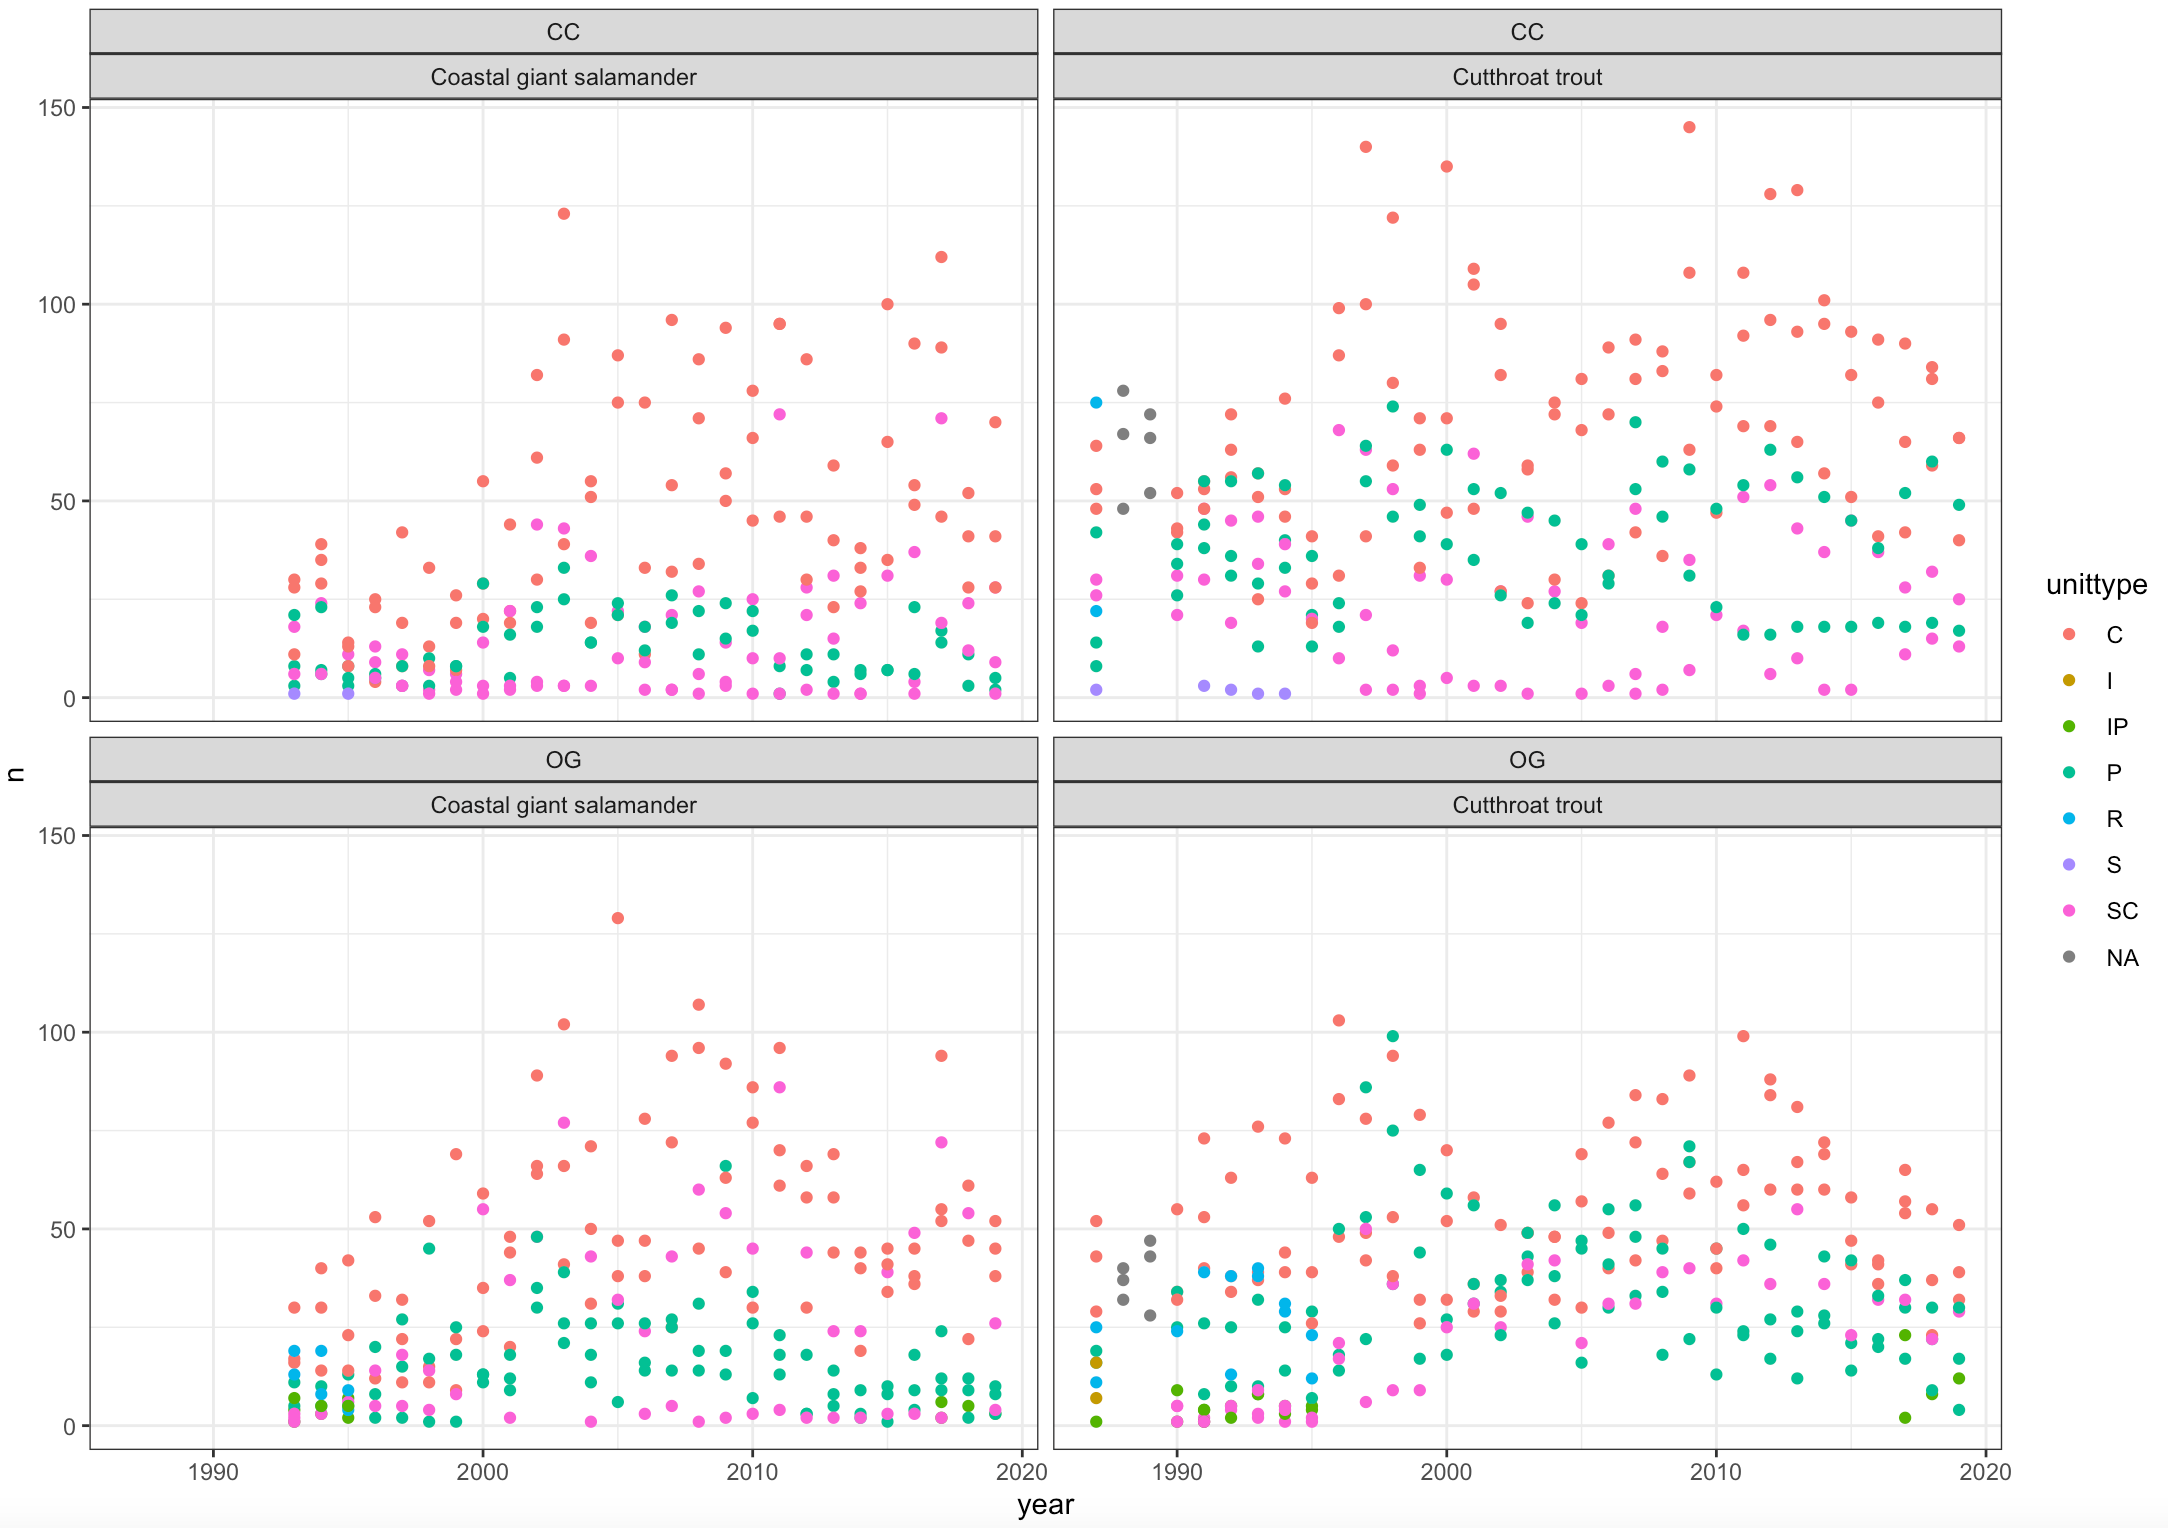
\includegraphics[width=0.9\linewidth]{figures/Screenshot 2023-03-05 at 11.09.31} \caption{Abundance by year, coloured by habitat}\label{fig:unnamed-chunk-13}
\end{figure}

This analytical process might have given us some idea of the abundances across year, reach and habitat type but its still pretty tricky to pull out much of a pattern from these data. So we need to do some more data wrangling to produce a plot that is more meaningful and easier to interpret. Look again at your plots, do you think that there are multiple data points per year and unittype? Could these be summarised more effectively by some measures of central tenancy and spread?

Try running the following to make a summary tibble;

\begin{Shaded}
\begin{Highlighting}[]
\NormalTok{summary }\OtherTok{\textless{}{-}}\NormalTok{ vert\_counts }\SpecialCharTok{\%\textgreater{}\%}
  \FunctionTok{group\_by}\NormalTok{(year, species, section, unittype) }\SpecialCharTok{\%\textgreater{}\%} 
  \FunctionTok{summarise}\NormalTok{(}\AttributeTok{mean=}\FunctionTok{mean}\NormalTok{(n),}
            \AttributeTok{sd=}\FunctionTok{sd}\NormalTok{(n),}
            \AttributeTok{n=}\FunctionTok{n}\NormalTok{())}
\NormalTok{summary}
\end{Highlighting}
\end{Shaded}

Have a look at the tibble produced, do you understand what each line of the above code has done? Try adding comments \texttt{\#} to your code.

It would also be useful to know the standard error of the mean as well. We can use the \texttt{mutate} function to add additional columns onto our summary stats table. Remember we can calculate the standard error of the mean using;

\[
SEM = \frac{SD}{\sqrt{n}}
\]
Add the following line of code to the end of the previous chunk, don't forget to include the piping syntax \texttt{\textgreater{}\%\textgreater{}};

\begin{Shaded}
\begin{Highlighting}[]
\FunctionTok{mutate}\NormalTok{(}\AttributeTok{sem =}\NormalTok{ sd}\SpecialCharTok{/}\FunctionTok{sqrt}\NormalTok{(n))}
\end{Highlighting}
\end{Shaded}

Your summary tibble should now look like this (note that this is just an exert, yours will be larger);

\begin{verbatim}
> summary
# A tibble: 386 × 8
# Groups:   year, species, section [120]
    year species         section unittype  mean    sd     n   sem
   <dbl> <chr>           <chr>   <chr>    <dbl> <dbl> <int> <dbl>
 1  1987 Cutthroat trout CC      C         55    8.19     3  4.73
 2  1987 Cutthroat trout CC      P         21.3 18.1      3 10.5 
 3  1987 Cutthroat trout CC      R         48.5 37.5      2 26.5 
 4  1987 Cutthroat trout CC      S          2   NA        1  NA   
 5  1987 Cutthroat trout CC      SC        28    2.83     2  2   
 6  1987 Cutthroat trout OG      C         41.3 11.6      3  6.69
 7  1987 Cutthroat trout OG      I         11.5  6.36     2  4.5 
\end{verbatim}

You might notice that there are some \texttt{NA} values stored here. This is because where there is only one data value per category combination (e.g.~1987, Cutthroat trout, CC, S) we cant calculate a standard deviation or a standard error of the mean. We don't want these \texttt{NA} values to cause future errors so we are just going to replace them with \texttt{0}. Add the this line to your last chunk (remember to pipe).

\begin{Shaded}
\begin{Highlighting}[]
\FunctionTok{mutate}\NormalTok{(}\AttributeTok{sem =} \FunctionTok{replace\_na}\NormalTok{(sem, }\DecValTok{0}\NormalTok{))}
\end{Highlighting}
\end{Shaded}

Now we can use this

\begin{Shaded}
\begin{Highlighting}[]
\NormalTok{summary }\SpecialCharTok{\%\textgreater{}\%}
  \FunctionTok{ggplot}\NormalTok{(}\FunctionTok{aes}\NormalTok{(}\AttributeTok{x =}\NormalTok{ year, }\AttributeTok{y =}\NormalTok{ mean, }\AttributeTok{colour =}\NormalTok{ unittype)) }\SpecialCharTok{+}
  \FunctionTok{geom\_line}\NormalTok{() }\SpecialCharTok{+}
  \FunctionTok{geom\_pointrange}\NormalTok{(}\FunctionTok{aes}\NormalTok{(}\AttributeTok{ymax =}\NormalTok{ mean}\SpecialCharTok{+}\NormalTok{sem, }\AttributeTok{ymin =}\NormalTok{ mean}\SpecialCharTok{{-}}\NormalTok{sem)) }\SpecialCharTok{+}
  \FunctionTok{theme\_bw}\NormalTok{() }\SpecialCharTok{+}
  \FunctionTok{facet\_wrap}\NormalTok{(section}\SpecialCharTok{\textasciitilde{}}\NormalTok{species)}
\end{Highlighting}
\end{Shaded}

To produce plots that look like this;

\begin{figure}
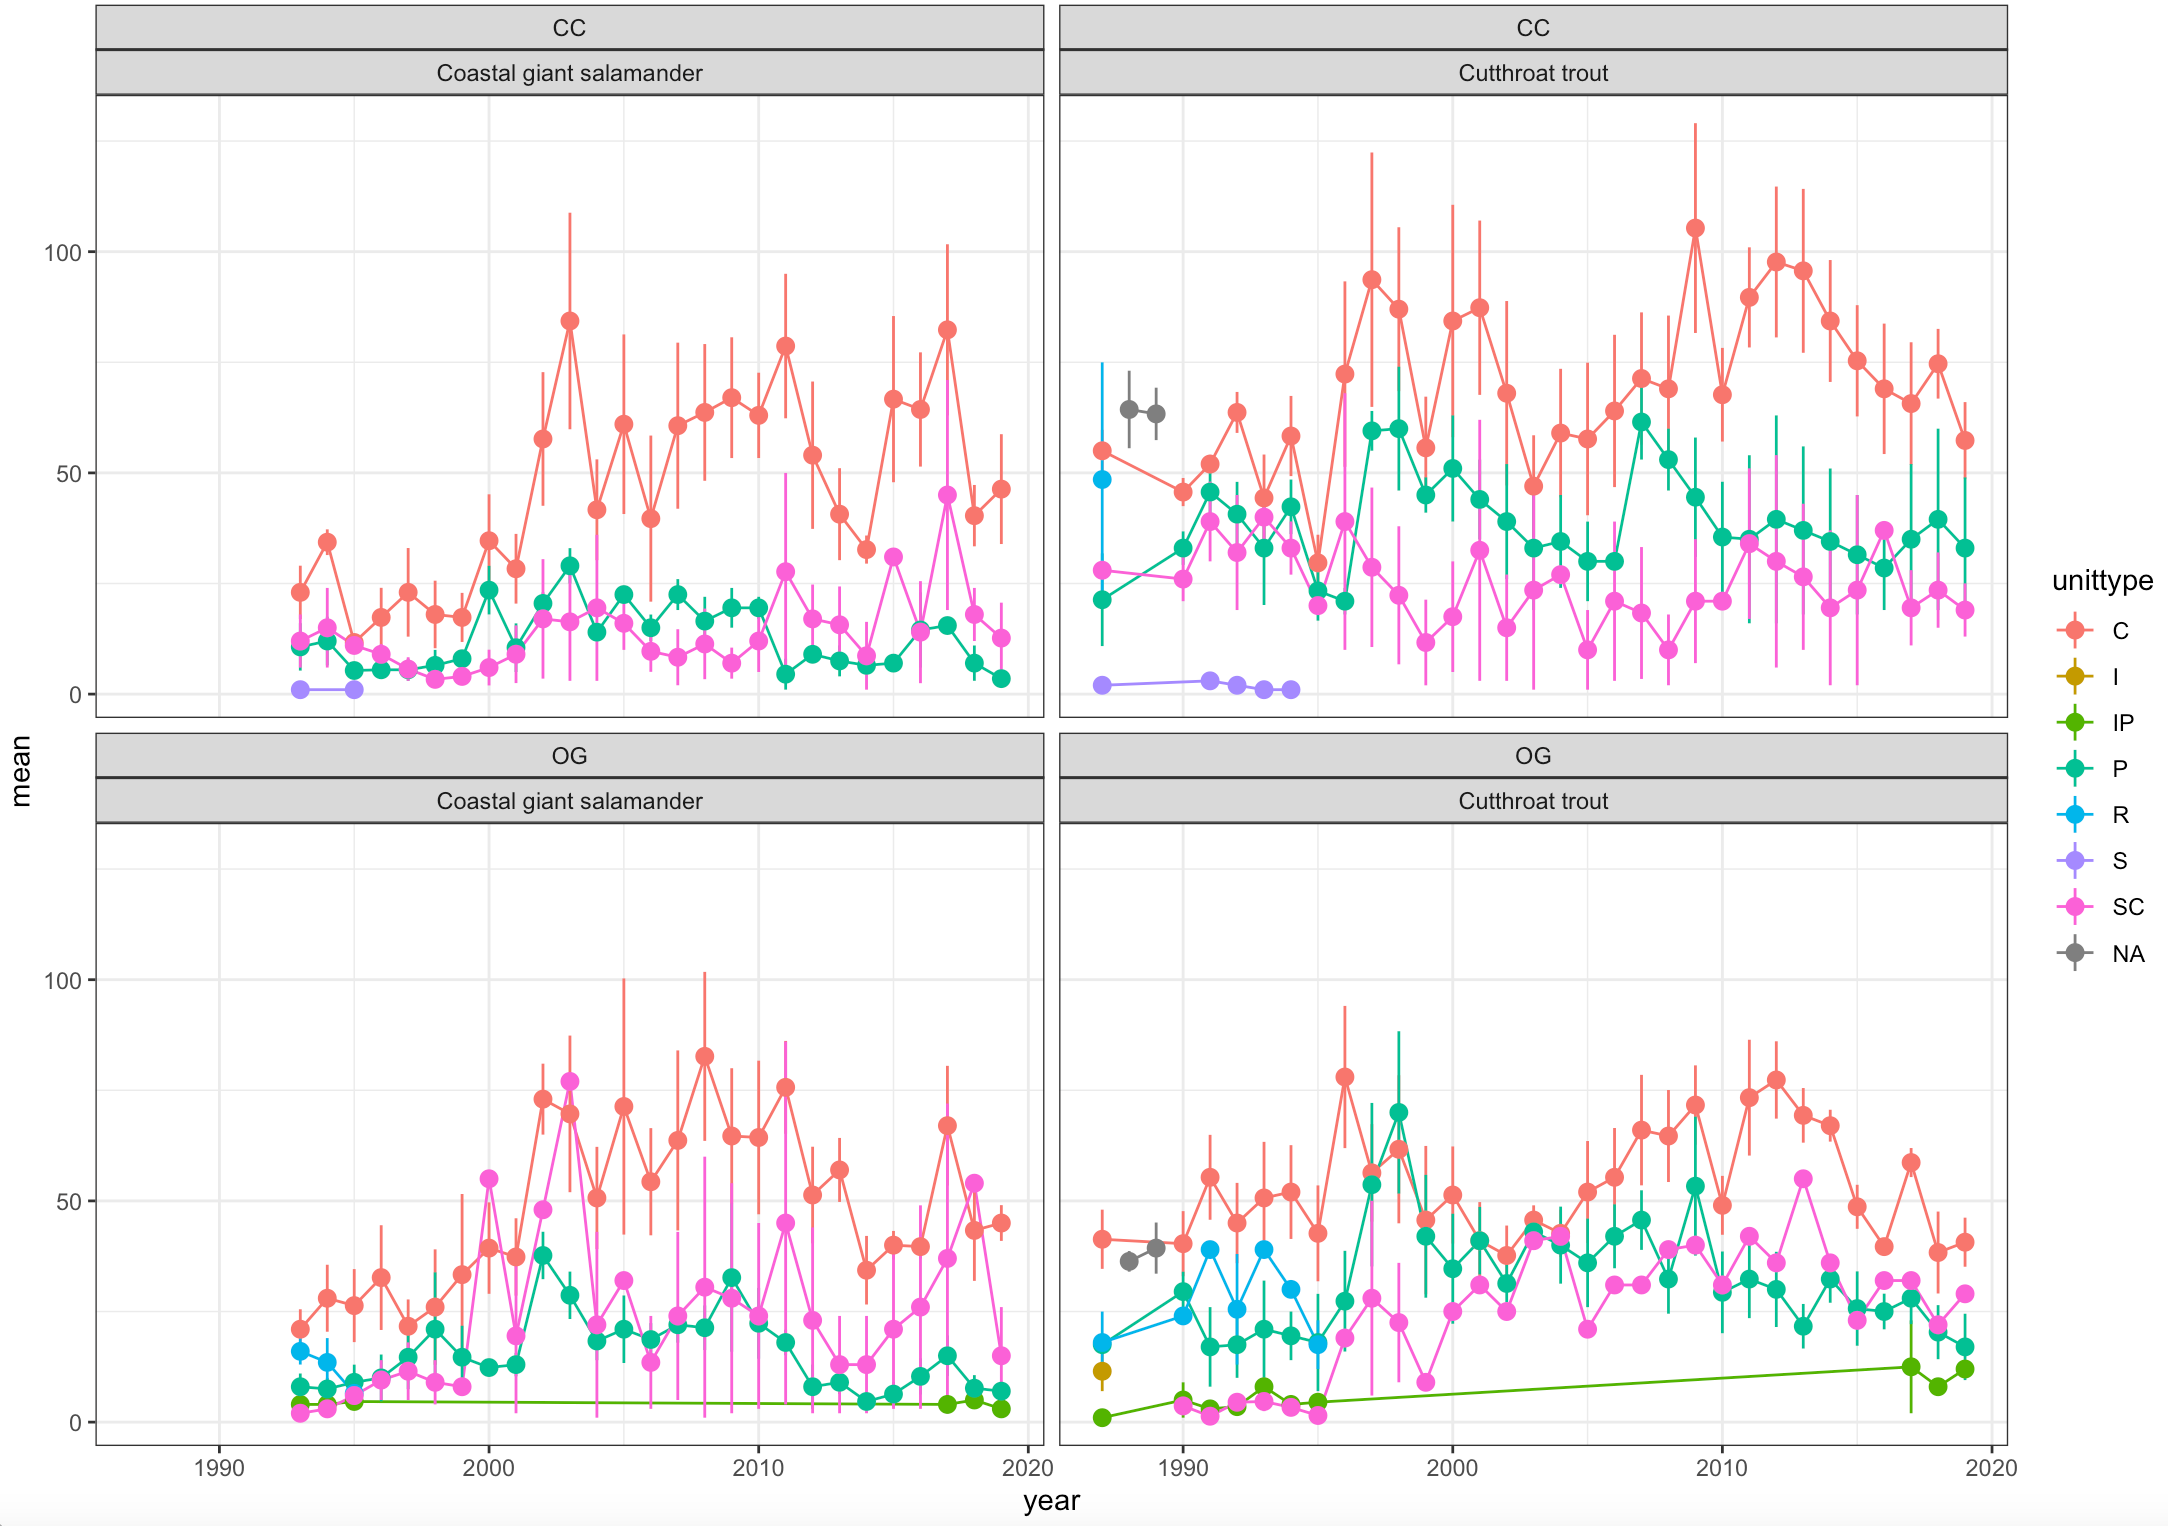
\includegraphics[width=0.9\linewidth]{figures/Screenshot 2023-03-05 at 12.12.37} \caption{Mean abundance by year, coloured by habitat}\label{fig:unnamed-chunk-18}
\end{figure}

Once again make sure you understand what each line of code has done, try adding comments \texttt{\#} to the script. Spend some time looking at these plots, what do they tell you? Remember that you have plotted mean and standard error for abundance across year, habitat, land management strategy and two species here, which gives you multiple questions you could ask of the data. It may be of interest to know that Mack Creek flooded in 1996. What impact (if any) did this have on our abundances? Remember to look at the variation in the data, don't just focus on the mean.

\begin{quote}
Note down some of your observations, interpretations or thoughts, we will have a class discussion around these in the last 20 minutes of the workshop.
\end{quote}

\hypertarget{comparing-habitat-and-land-management-strategy-impacts-on-abundance}{%
\section{Comparing habitat and land management strategy impacts on abundance}\label{comparing-habitat-and-land-management-strategy-impacts-on-abundance}}

We may wish to directly compare abundances between habitat and land management strategy (removing time as a variable). How do you think you might go about this? See if you can manipulate some of the above scripts to produce an appropriate plot;

\begin{quote}
Hint - I would use geom\_boxplot
\end{quote}

What do these new plots tell you about differences in abundance in either trout or salamander species between different habitats/land management strategy?

\begin{quote}
Note down some of your observations, interpretations or thoughts, we will have a class discussion around these in the last 20 minutes of the workshop.
\end{quote}

\hypertarget{bonus-challenge}{%
\section{Bonus Challenge}\label{bonus-challenge}}

Our original data set also contained data on salamander and trout standard length and weight. Have a go at exploring these data, do you think habitat or land management has any impact on the biomass of trout or salamanders? Think about the most appropriate plots you could produce to explore these questions.

\begin{quote}
Note down some of your observations, interpretations or thoughts, we will have a class discussion around these in the last 20 minutes of the workshop.
\end{quote}

\hypertarget{discussion}{%
\section{Discussion}\label{discussion}}

The last 20 minutes of this session will be used for a class discussion around the observations you have made from the plots produced. Think about any major patterns that have emerged, can you link these patterns back to any one single variable?

\hypertarget{before-you-leave}{%
\section{Before you leave}\label{before-you-leave}}

Please log out of posit Cloud before you leave and make sure you save your script, we will come back to it in future workshops.

\hypertarget{references}{%
\chapter{References}\label{references}}

Gregory, S.V. and Arismendi, I. (2020). Aquatic Vertebrate Population Study in Mack Creek, Andrews Experimental Forest, 1987 to present ver 14. Environmental Data Initiative. \url{https://doi.org/10.6073/pasta/7c78d662e847cdbe33584add8f809165}
Horst A., Brun J. (2023). lterdatasampler: Educational dataset examples from the Long Term Ecological Research program. R package version 0.1.1, \url{https://github.com/lter/lterdatasampler}.
Kaylor. M. and Warren, D. (2017) Linking riparian shade and the legacies of forest management to fish and vertebrate biomass in forested streams. Ecosphere, 8(6), e01845. \url{https://doi.org/10.1002/ecs2.1845}
Wickham, H., Averick, M., Bryan, j., Chang, W., D'Agostino McGowan , L., François, R., Grolemund, G. (2019). ``Welcome to the tidyverse.'' Journal of Open Source Software 4 (43): 1686. \url{https://doi.org/10.21105/joss.01686}.

\end{document}
